% Warns the user when LateX is wrongly used
% http://www.ctan.org/tex-archive/macros/latex/contrib/nag
\RequirePackage[l2tabu, orthodox]{nag}

% http://www.ctan.org/pkg/scrreprt
\documentclass[
    pagesize=pdftex,    % Page size is set with \pdfpagewidth and \pdfpageheight
    twoside=false,      % Einseitiger Druck.
    fontsize=12pt,      % Schriftgroesse
    parskip=half,       % Halbe Zeile Abstand zwischen Absätzen.
    headsepline,        % Linie nach Kopfzeile.
    footsepline,        % Linie vor Fusszeile.
    abstract=false,     % Abstract Überschriften
    listof=totoc,       % show table of figures in toc but unnumbered
    toc=bibliography,   % show bibliography in toc but unnumbered
]{scrreprt}

\usepackage{special-generated/customsettings}

\title{Systemnahe Programmierung}
\author{}
\date{\today}

% Support for hypertext links
% http://www.ctan.org/pkg/hyperref
\usepackage[%
    pdftitle={Systemnahe Programmierung},                % text for PDF Title field 
    pdfauthor={},              % text for PDF Author field 
    pdfsubject={Systemnahe Programmierung},              % text for PDF Subject field 
    pdfcreator={pdflatex, LaTeX with KOMA-Script},   % text for PDF Creator field 
    pdfpagemode=UseOutlines,        % show bookmarks
    pdflang={de},                   % language identifier (RFC 3066)
    hidelinks,                      % hide links (no color, no border)
    bookmarksnumbered=true,         % put section numbers in bookmarks
    pdfdisplaydoctitle=true,        % display document title instead of file name in title bar
]{hyperref}

% A new bookmark (outline) organization for package hyperref
% bookmarks are generated on first compile
% http://www.ctan.org/pkg/bookmark
% \usepackage{bookmark}

%%% New commands.

% Don't output references in case they're empty
% http://tex.stackexchange.com/questions/74476/how-to-avoid-empty-thebibliography-environment-bibtex-if-there-are-no-refere



% Stdfig -> Used as \stdfig{width}{label_name}{caption}
% Requires: image called 'caption' in img folder.
% Output: A figure with the given width, labeled as 'fig:label_name'

\newcommand{\stdfig}[3]{
    \begin{figure}
    \centering
    \includegraphics[width = #1]{img/#2.eps}
    \caption{#3}
    \label{fig:#2}
    \end{figure}
}



% inplacefig -> Used as \inplacefig{width}{img_name}
% Requires: image called 'img_name' in img folder.
% Output: an inplace figure with the given width, labeled as 'fig:label_name'.

\newcommand{\inplacefig}[2]{
    \begin{figure}[H]
    \centering
    \includegraphics[width = #1]{img/#2.eps}
    \label{fig:#2}
    \end{figure}
}


%\makeglossaries
%%!TEX root = ../dokumentation.tex

%
% vorher in Konsole folgendes aufrufen:
%	makeglossaries makeglossaries dokumentation.acn && makeglossaries dokumentation.glo
%

%
% Glossareintraege --> referenz, name, beschreibung
% Aufruf mit \gls{...}
%
\newglossaryentry{Glossareintrag}{name={Glossareintrag},plural={Glossareinträge},description={Ein Glossar beschreibt verschiedenste Dinge in kurzen Worten}}


\begin{document}


\selectlanguage{ngerman}



%% Front page.
\title{Systemnahe Programmierung}



\author{
        Julien Hadley Jack \\
        Sebastian Dernbach \\
       }


\maketitle

\newpage



% Inhaltsverzeichnis
\pagestyle{plain}
%für die Anzeige von Unterkapiteln im Inhaltsverzeichnis: 2
\setcounter{tocdepth}{2}
\tableofcontents
\newpage



%% Body start.
%!TEX root = ../systemnahe-programmierung.tex

\chapter{Einleitung}\label{einleitung}

\begin{figure}[htbp]
\centering
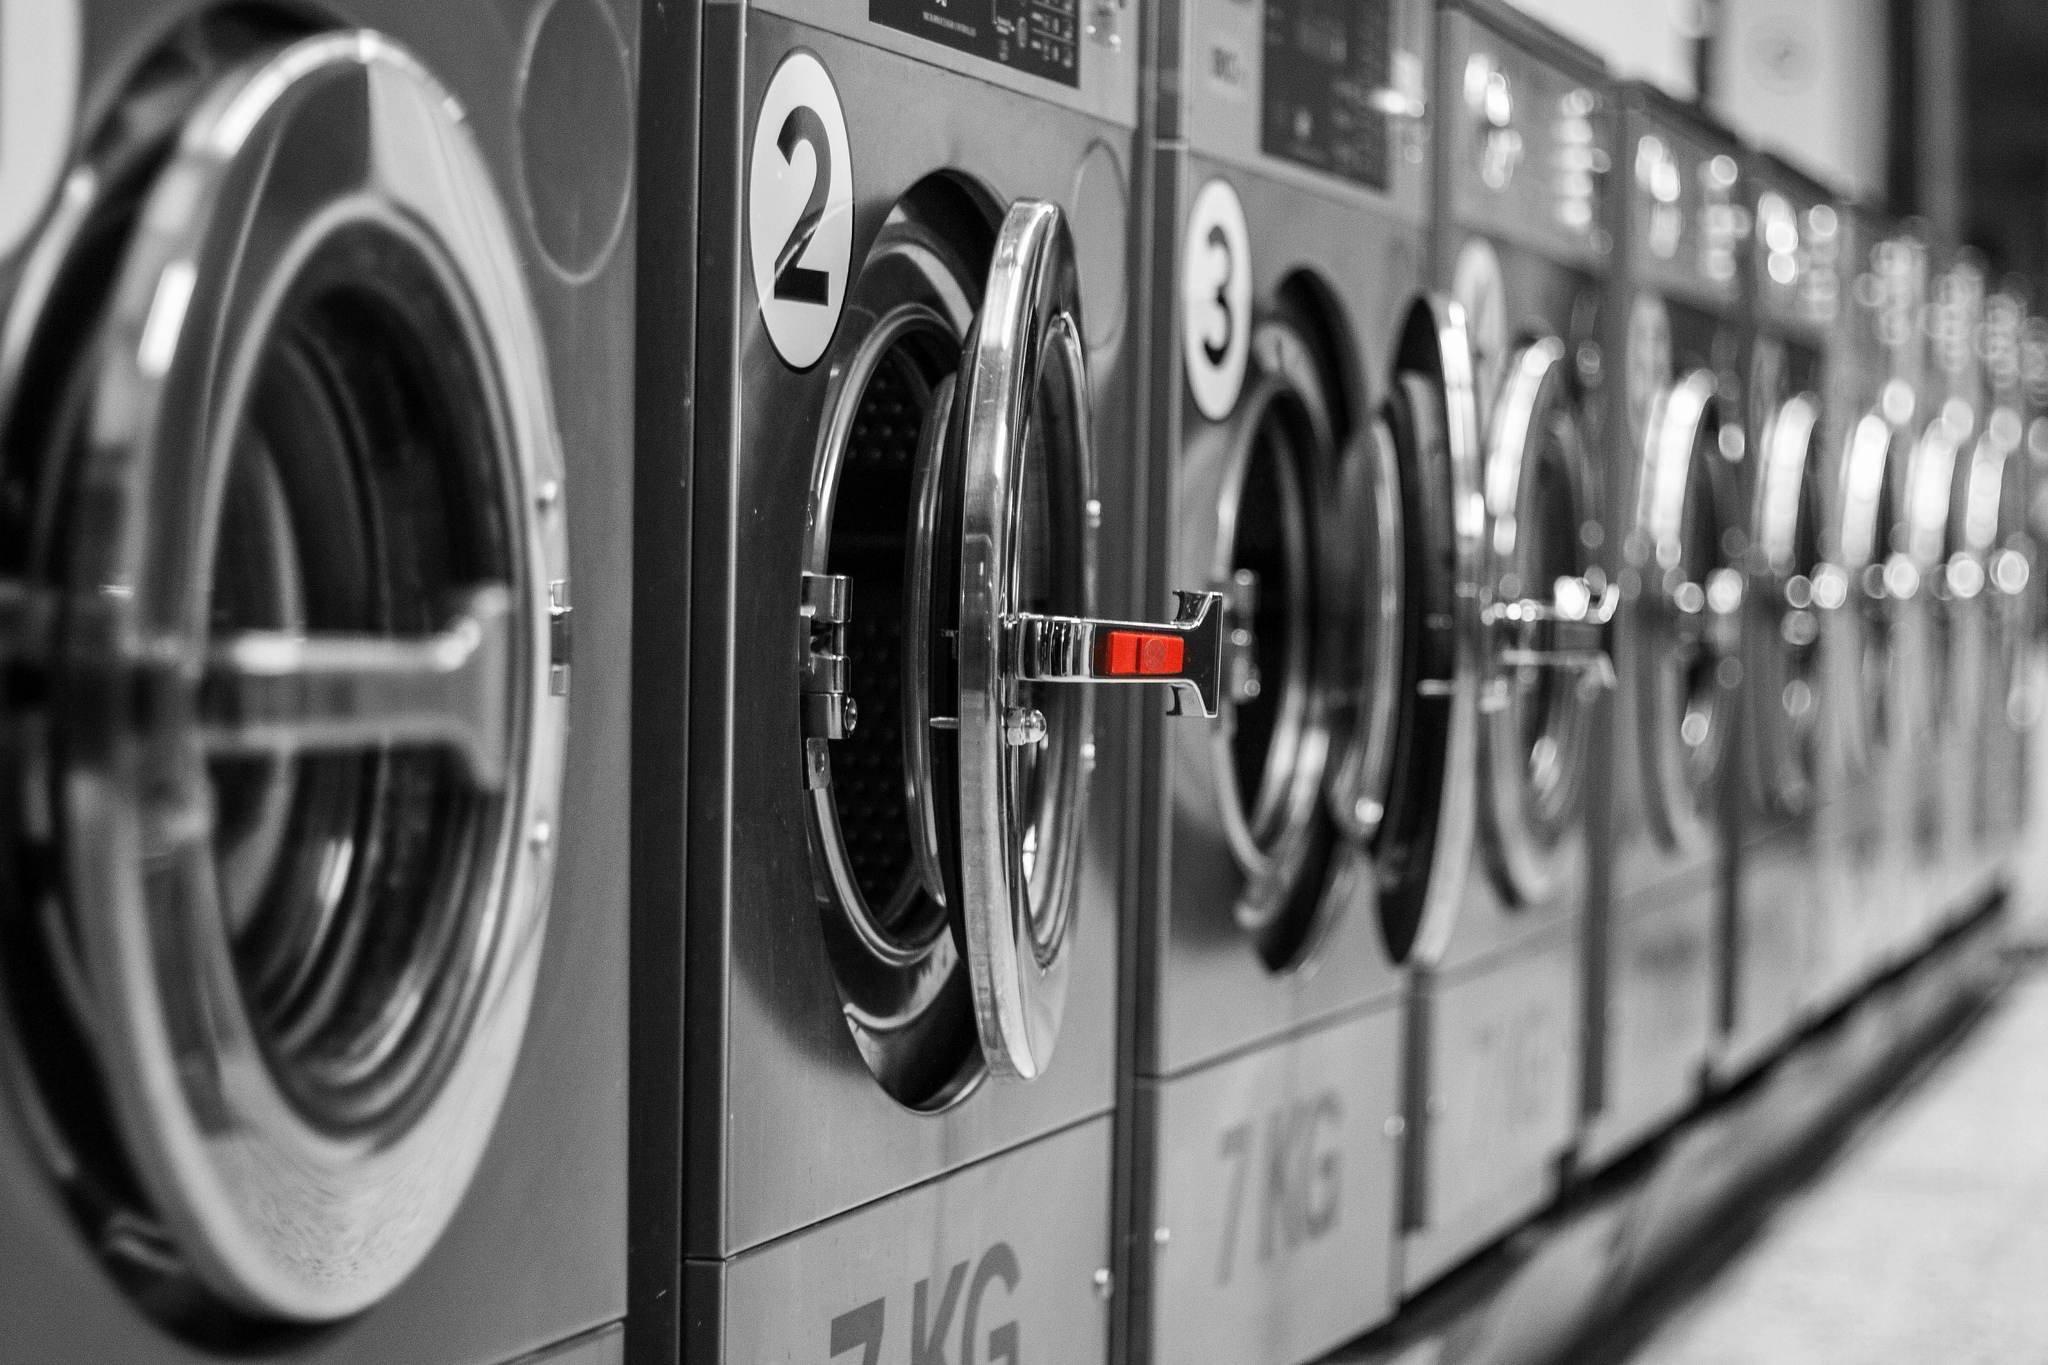
\includegraphics{images/washing-maschine}
\caption[Microcontroller im Alltag]{Microcontroller im Alltag\footnotemark{}}
\end{figure}
\footnotetext{Choose only one, https://www.flickr.com/photos/97922031@N05/15884820461,
  Einsichtsnahme: 31.01.2015}

Systemnahe Programmierung beschäftigt sich mit der Erstellung beziehungsweise Programmierung von
Software, die Teil des Betriebssystemes oder sehr eng mit diesem verbunden ist.

Die Software dient hierbei als Abstraktionsschicht zwischen Hardware und Betriebssystem, welche
leichten Zugriff auf einfache Funktionen des Systems bietet.

Heutzutage nimmt Systemnahe Programmierung einen sehr hohen Stellenwert ein. Sie ist mittlerweile in
unserem Alltag in Form von Microcontrollern mit verschiedensten Einsatzgebieten vertreten.
Microcontroller sind in Autos, Mobiltelefonen, Waschmaschinen, elektrischen Zahnbürsten,
Fernbedienungen und vielen anderen Geräten zu finden.

Die Systeme sind nicht nur omnipräsent sondern der Markt wächst immer mehr. Durch den Aufstieg von
Wearables und dem Drang alle Geräte miteinander zu verbinden, werden immer mehr Microcontroller
verbaut. So kam auch der Anstieg von 12\% in 2014 zu Stande, der für 2015 mit 15\% noch höher
ausfallen soll\footnote{(o.V.) (2015) Microcontroller market 2015,
  http://www.emittsolutions.com/section/market-analysis/market\_analysis\_microcontroller.html,
  Einsichtnahme: 27.01.2015.}.
%!TEX root = ../systemnahe-programmierung.tex

\chapter{Geschichte}\label{geschichte}

\begin{figure}[htbp]
\centering
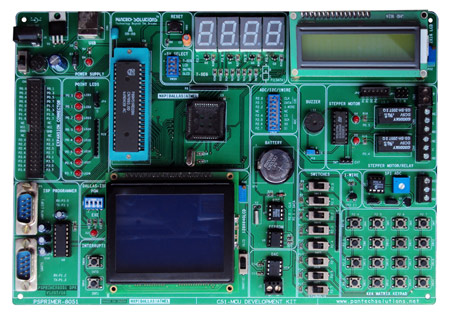
\includegraphics{images/8051-board}
\caption[8051 Board ]{8051 Board \footnotemark{}}
\end{figure}
\footnotetext{8051 Primer Board, https://www.flickr.com/photos/pantechsolutions/5760938387,
  Einsichtsnahme: 31.01.2015}

1980 präsentierte Intel den Nachfolger des 8048, den 8051. Er war als Erweiterung des 8048 zu sehen,
wurde von Intel intern als ``Verbesserte MCS-48 Architektur'' bezeichnent und enthielt somit
jegliche Funktionen dessen. Unteranderem wurden die Anzahl der Register mit 4 verdoppelt, ein
zweiter Timer eingeführt und diese auf 16-Bit aufgestockt.

Zum großen Erfolg des 8051 trug Intel mit den von Start ab vohandenen nötigen Programmen (Assembler,
Emulator, Software Beispielen) und der ausführlichen Dokumentation bei. So kamen bald verschiedene
Varianten ohne \ac{ROM} (8031) oder mit \ac{EPROM} (8751) auf und wurden bald durch noch bessere
Versionen mit mehr \ac{ROM}, \ac{RAM} und Timern ersetzt (z.B. 8052, 8kB \ac{ROM}, 256B \ac{RAM}, 3
16-Bit Timer). Durch die Lizensierung verschiedenster Firmen zur Herstellung des 8051 entstanden
immer mehr Varianten des ursprünglichen Microcontrollers. So z.B. in den 90ern Varianten mit Flash
Speicher um für Fehlerbehebungen oder neue Funktionen neu programmiert werden konnten und somit die
Kosten senkten.

Mit der großen Aktzeptanz des 8051 wurden die Applikationen immer größer und benötigten somit auch
mehr Leistung. Diese sollte eine 16-Bit Version des Controllers mit sich bringen, die kompatibel zur
ursprünglichen Version war. Nach dem Misserfolg dieser Variante konnten erst später Dritthersteller
eine erfolgreiche Variante mit mehr Megaherz auf den Markt bringen.
%!TEX root = ../systemnahe-programmierung.tex

\chapter{Mikrocontroller-Architektur}\label{mikrocontroller-architektur}

Bei der Intel 8051 Familie handelt es sich um einen 8-Bit Prozessorkern mit einem einheitlichen
Befehlssatz. Es werden 128 Byte \ac{RAM} und 4096 Byte \ac{ROM} intern verbaut, wobei die
Möglichkeit zum Anschluss von externem \ac{RAM} und \ac{ROM} besteht. Außerdem besitzt er 2 Timer
und 4 8-bit \ac{I/O} Ports. Sie besitzt 2 externe Interrupt Quellen sowie 2 verschiedene Interrupt
Prioritäten.

Als Datenspeicher dienen die 8 Register, aufgeteilt auf die 4 Registerbänke. Diese sind direkt über
ihre Adresse oder als reguläres Register ansprechbar. Als Programmspeicher kann entweder der interne
oder der externe Speicher verwendet werden.

Zur Ausführung eines Befehls benötigt der 8051 mindestens 12 Takte. Durch die Trennung von Befehls-
und Datenspeicher ist die Harvard Architektur zu erkennen.
%!TEX root = ../systemnahe-programmierung.tex

\chapter{Befehlssatz}\label{befehlssatz}

Dies ist ein Ausszug aus dem Befehlssatz\footnote{(o.V.) (o.J.) alle
  Befehle der 8051-Mikrocontroller-Familie,
  http://www.self8051.de/alle-Befehle-des-8051-Mikrocontroller,13290.html,
  Einsichtnahme: 27.01.2015.}.

\begin{longtable}[c]{@{}ll@{}}
\toprule
\begin{minipage}[b]{0.25\columnwidth}\raggedright\strut
\textbf{Befehl}
\strut\end{minipage} &
\begin{minipage}[b]{0.69\columnwidth}\raggedright\strut
\textbf{Beschreibung}
\strut\end{minipage}\tabularnewline
\midrule
\endhead
\begin{minipage}[t]{0.25\columnwidth}\raggedright\strut
\texttt{ACALL\ \textless{}addr11\textgreater{}}
\strut\end{minipage} &
\begin{minipage}[t]{0.69\columnwidth}\raggedright\strut
Ruft die Subroutine an der Adresse
\texttt{\textless{}addr11\textgreater{}} auf
\strut\end{minipage}\tabularnewline
\begin{minipage}[t]{0.25\columnwidth}\raggedright\strut
\texttt{ADD\ \textless{}A\textgreater{},\textless{}Operand\textgreater{}}
\strut\end{minipage} &
\begin{minipage}[t]{0.69\columnwidth}\raggedright\strut
Addiert den \texttt{\textless{}Operand\textgreater{}} zum Inhalt des
Akkumulators \texttt{\textless{}A\textgreater{}} hinzu
\strut\end{minipage}\tabularnewline
\begin{minipage}[t]{0.25\columnwidth}\raggedright\strut
\texttt{ADDC\ \textless{}A\textgreater{},\textless{}Operand\textgreater{}}
\strut\end{minipage} &
\begin{minipage}[t]{0.69\columnwidth}\raggedright\strut
Addiert den \texttt{\textless{}Operand\textgreater{}} und das
Übertragsbit zum Inhalt des Akkumulators
\texttt{\textless{}A\textgreater{}} hinzu
\strut\end{minipage}\tabularnewline
\begin{minipage}[t]{0.25\columnwidth}\raggedright\strut
\texttt{AJMP\ \textless{}addr11\textgreater{}}
\strut\end{minipage} &
\begin{minipage}[t]{0.69\columnwidth}\raggedright\strut
Springt zu Adresse \texttt{\textless{}addr11\textgreater{}}
\strut\end{minipage}\tabularnewline
\begin{minipage}[t]{0.25\columnwidth}\raggedright\strut
\texttt{ANL\ \textless{}Zielbyte\textgreater{},\ \textless{}Quellenbyte\textgreater{}}
\strut\end{minipage} &
\begin{minipage}[t]{0.69\columnwidth}\raggedright\strut
Speichert eine bitweise logische UND-Verknüpfung zwischen dem
\texttt{\textless{}Zielbyte\textgreater{}} und dem
\texttt{\textless{}Quellenbyte\textgreater{}} im
\texttt{\textless{}Zielbyte\textgreater{}}
\strut\end{minipage}\tabularnewline
\begin{minipage}[t]{0.25\columnwidth}\raggedright\strut
\texttt{CJNE\ \textless{}Operand1\textgreater{},}
\texttt{\textless{}Operand2\textgreater{},\textless{}rel\textgreater{}}
\strut\end{minipage} &
\begin{minipage}[t]{0.69\columnwidth}\raggedright\strut
Springe zu \texttt{\textless{}rel\textgreater{}} falls die Werte
\texttt{\textless{}Operand1\textgreater{}} und
\texttt{\textless{}Operand2\textgreater{}} ungleich sind
\strut\end{minipage}\tabularnewline
\begin{minipage}[t]{0.25\columnwidth}\raggedright\strut
\texttt{CLR\ \textless{}bit\textgreater{}/\textless{}A\textgreater{}}
\strut\end{minipage} &
\begin{minipage}[t]{0.69\columnwidth}\raggedright\strut
Löscht das Bit \texttt{\textless{}bit\textgreater{}} bzw. den
Akkumulator \texttt{\textless{}A\textgreater{}}
\strut\end{minipage}\tabularnewline
\begin{minipage}[t]{0.25\columnwidth}\raggedright\strut
\texttt{CPL\ \textless{}bit\textgreater{}/\textless{}A\textgreater{}}
\strut\end{minipage} &
\begin{minipage}[t]{0.69\columnwidth}\raggedright\strut
Komplementiert das Bit \texttt{\textless{}bit\textgreater{}} bzw. den
Akkumulator \texttt{\textless{}A\textgreater{}}
\strut\end{minipage}\tabularnewline
\begin{minipage}[t]{0.25\columnwidth}\raggedright\strut
\texttt{DA\ \textless{}A\textgreater{}}
\strut\end{minipage} &
\begin{minipage}[t]{0.69\columnwidth}\raggedright\strut
Korrigiere den Dezimalwert des Akkumulators
\texttt{\textless{}A\textgreater{}} nach einer Addition
\strut\end{minipage}\tabularnewline
\begin{minipage}[t]{0.25\columnwidth}\raggedright\strut
\texttt{DEC\ \textless{}byte\textgreater{}}
\strut\end{minipage} &
\begin{minipage}[t]{0.69\columnwidth}\raggedright\strut
Dekrementiere \texttt{\textless{}byte\textgreater{}} um 1
\strut\end{minipage}\tabularnewline
\begin{minipage}[t]{0.25\columnwidth}\raggedright\strut
\texttt{DIV\ \textless{}A\textgreater{},\textless{}B\textgreater{}}
\strut\end{minipage} &
\begin{minipage}[t]{0.69\columnwidth}\raggedright\strut
Dividiere Akkumulator \texttt{\textless{}A\textgreater{}} durch Register
\texttt{\textless{}B\textgreater{}}
\strut\end{minipage}\tabularnewline
\begin{minipage}[t]{0.25\columnwidth}\raggedright\strut
\texttt{DJNZ\ \textless{}byte\textgreater{},\textless{}rel\textgreater{}}
\strut\end{minipage} &
\begin{minipage}[t]{0.69\columnwidth}\raggedright\strut
Dekrementiere \texttt{\textless{}byte\textgreater{}} um 1 und springe zu
\texttt{\textless{}rel\textgreater{}} wenn das
\texttt{\textless{}byte\textgreater{}} nicht Null ist
\strut\end{minipage}\tabularnewline
\begin{minipage}[t]{0.25\columnwidth}\raggedright\strut
\texttt{INC\ \textless{}byte\textgreater{}/\textless{}DPTR\textgreater{}}
\strut\end{minipage} &
\begin{minipage}[t]{0.69\columnwidth}\raggedright\strut
Inkrementiere \texttt{\textless{}byte\textgreater{}} bzw.
\texttt{\textless{}DPTR\textgreater{}} um 1
\strut\end{minipage}\tabularnewline
\begin{minipage}[t]{0.25\columnwidth}\raggedright\strut
\texttt{JB\ \textless{}bit\textgreater{},\textless{}rel\textgreater{}}
\strut\end{minipage} &
\begin{minipage}[t]{0.69\columnwidth}\raggedright\strut
Springe zu \texttt{\textless{}rel\textgreater{}}, wenn
\texttt{\textless{}byte\textgreater{}} gesetzt ist (=1)
\strut\end{minipage}\tabularnewline
\begin{minipage}[t]{0.25\columnwidth}\raggedright\strut
\texttt{JBC\ \textless{}bit\textgreater{},\textless{}rel\textgreater{}}
\strut\end{minipage} &
\begin{minipage}[t]{0.69\columnwidth}\raggedright\strut
Springe zu \texttt{\textless{}rel\textgreater{}}, wenn
\texttt{\textless{}byte\textgreater{}} gesetzt ist (=1) und lösche
dieses anschließend
\strut\end{minipage}\tabularnewline
\begin{minipage}[t]{0.25\columnwidth}\raggedright\strut
\texttt{JC\ \textless{}rel\textgreater{}}
\strut\end{minipage} &
\begin{minipage}[t]{0.69\columnwidth}\raggedright\strut
Springe zu \texttt{\textless{}rel\textgreater{}}, wenn das Übertragsbit
gesetzt ist (=1)
\strut\end{minipage}\tabularnewline
\begin{minipage}[t]{0.25\columnwidth}\raggedright\strut
\texttt{JMP\ \textless{}A\textgreater{}+\textless{}DPTR\textgreater{}}
\strut\end{minipage} &
\begin{minipage}[t]{0.69\columnwidth}\raggedright\strut
Addiere den Akkumulator \texttt{\textless{}A\textgreater{}} zum
Datenanzeiger \texttt{\textless{}DPTR\textgreater{}} und lade das
Ergebnis in den Programmzähler
\strut\end{minipage}\tabularnewline
\begin{minipage}[t]{0.25\columnwidth}\raggedright\strut
\texttt{JNB\ \textless{}bit\textgreater{},\textless{}rel\textgreater{}}
\strut\end{minipage} &
\begin{minipage}[t]{0.69\columnwidth}\raggedright\strut
Springe zu \texttt{\textless{}rel\textgreater{}}, wenn
\texttt{\textless{}byte\textgreater{}} nicht gesetzt ist (=0)
\strut\end{minipage}\tabularnewline
\begin{minipage}[t]{0.25\columnwidth}\raggedright\strut
\texttt{JNC\ \textless{}rel\textgreater{}}
\strut\end{minipage} &
\begin{minipage}[t]{0.69\columnwidth}\raggedright\strut
Springe zu \texttt{\textless{}rel\textgreater{}}, wenn das Übertragsbit
nicht gesetzt ist (=0)
\strut\end{minipage}\tabularnewline
\begin{minipage}[t]{0.25\columnwidth}\raggedright\strut
\texttt{JNZ\ \textless{}rel\textgreater{}}
\strut\end{minipage} &
\begin{minipage}[t]{0.69\columnwidth}\raggedright\strut
Springe zu \texttt{\textless{}rel\textgreater{}}, wenn der Akkumulator
nicht Null ist
\strut\end{minipage}\tabularnewline
\begin{minipage}[t]{0.25\columnwidth}\raggedright\strut
\texttt{JZ\ \textless{}rel\textgreater{}}
\strut\end{minipage} &
\begin{minipage}[t]{0.69\columnwidth}\raggedright\strut
Springe zu \texttt{\textless{}rel\textgreater{}}, wenn der Akkumulator
Null ist
\strut\end{minipage}\tabularnewline
\begin{minipage}[t]{0.25\columnwidth}\raggedright\strut
\texttt{LCALL\ \textless{}addr16\textgreater{}}
\strut\end{minipage} &
\begin{minipage}[t]{0.69\columnwidth}\raggedright\strut
Ruft bedingungslos Subroutine an der Adresse
\texttt{\textless{}addr16\textgreater{}} auf
\strut\end{minipage}\tabularnewline
\begin{minipage}[t]{0.25\columnwidth}\raggedright\strut
\texttt{LJMP\ \textless{}addr16\textgreater{}}
\strut\end{minipage} &
\begin{minipage}[t]{0.69\columnwidth}\raggedright\strut
Springt bedingungslos zur Adresse
\texttt{\textless{}addr16\textgreater{}}
\strut\end{minipage}\tabularnewline
\begin{minipage}[t]{0.25\columnwidth}\raggedright\strut
\texttt{MOV\ \textless{}Zielbyte\textgreater{},}
\texttt{\textless{}Quellenbyte\textgreater{}}
\strut\end{minipage} &
\begin{minipage}[t]{0.69\columnwidth}\raggedright\strut
Kopiere das \texttt{\textless{}Quellenbyte\textgreater{}} in das
\texttt{\textless{}Zielbyte\textgreater{}}
\strut\end{minipage}\tabularnewline
\begin{minipage}[t]{0.25\columnwidth}\raggedright\strut
\texttt{MOV\ \textless{}Zielbit\textgreater{},}
\texttt{\textless{}Quellenbit\textgreater{}}
\strut\end{minipage} &
\begin{minipage}[t]{0.69\columnwidth}\raggedright\strut
Kopiere das \texttt{\textless{}Quellenbit\textgreater{}} in das
\texttt{\textless{}Zielbit\textgreater{}}
\strut\end{minipage}\tabularnewline
\begin{minipage}[t]{0.25\columnwidth}\raggedright\strut
\texttt{MOV\ \textless{}DPTR\textgreater{},\textless{}data16\textgreater{}}
\strut\end{minipage} &
\begin{minipage}[t]{0.69\columnwidth}\raggedright\strut
Lade die Konstante \texttt{\textless{}data16\textgreater{}} in den
Datenzeiger \texttt{\textless{}DPTR\textgreater{}}
\strut\end{minipage}\tabularnewline
\begin{minipage}[t]{0.25\columnwidth}\raggedright\strut
\texttt{MUL\ \textless{}A\textgreater{},\textless{}B\textgreater{}}
\strut\end{minipage} &
\begin{minipage}[t]{0.69\columnwidth}\raggedright\strut
Multipliziere den Akkumulator \texttt{\textless{}A\textgreater{}} zum
Register \texttt{\textless{}B\textgreater{}}
\strut\end{minipage}\tabularnewline
\begin{minipage}[t]{0.25\columnwidth}\raggedright\strut
\texttt{NOP}
\strut\end{minipage} &
\begin{minipage}[t]{0.69\columnwidth}\raggedright\strut
Setze Programm mit folgendem Befehl fort
\strut\end{minipage}\tabularnewline
\begin{minipage}[t]{0.25\columnwidth}\raggedright\strut
\texttt{ORL\ \textless{}Zielbyte\textgreater{},}
\texttt{\textless{}Quellenbyte\textgreater{}}
\strut\end{minipage} &
\begin{minipage}[t]{0.69\columnwidth}\raggedright\strut
Speichert eine bitweise logische ODER-Verknüpfung zwischen dem
\texttt{\textless{}Zielbyte\textgreater{}} und dem
\texttt{\textless{}Quellenbyte\textgreater{}} im
\texttt{\textless{}Zielbyte\textgreater{}}
\strut\end{minipage}\tabularnewline
\begin{minipage}[t]{0.25\columnwidth}\raggedright\strut
\texttt{POP\ \textless{}byte\textgreater{}}
\strut\end{minipage} &
\begin{minipage}[t]{0.69\columnwidth}\raggedright\strut
Bringe den Wert vom Stack Pointer zum Byte
\texttt{\textless{}byte\textgreater{}} und dekrementiere den Stack
Pointer
\strut\end{minipage}\tabularnewline
\begin{minipage}[t]{0.25\columnwidth}\raggedright\strut
\texttt{PUSH\ \textless{}byte\textgreater{}}
\strut\end{minipage} &
\begin{minipage}[t]{0.69\columnwidth}\raggedright\strut
Kopiere den Wert vom Byte \texttt{\textless{}byte\textgreater{}} in den
Stack Pointer und inkrementiere den Stack Pointer
\strut\end{minipage}\tabularnewline
\begin{minipage}[t]{0.25\columnwidth}\raggedright\strut
\texttt{RET}
\strut\end{minipage} &
\begin{minipage}[t]{0.69\columnwidth}\raggedright\strut
Springt aus der Subroutine zurück
\strut\end{minipage}\tabularnewline
\begin{minipage}[t]{0.25\columnwidth}\raggedright\strut
\texttt{RETI}
\strut\end{minipage} &
\begin{minipage}[t]{0.69\columnwidth}\raggedright\strut
Springe aus dem Interrupt zurück
\strut\end{minipage}\tabularnewline
\begin{minipage}[t]{0.25\columnwidth}\raggedright\strut
\texttt{RL\ \textless{}A\textgreater{}}
\strut\end{minipage} &
\begin{minipage}[t]{0.69\columnwidth}\raggedright\strut
Schiebe die Bits des Akkumulators \texttt{\textless{}A\textgreater{}}
nach links
\strut\end{minipage}\tabularnewline
\begin{minipage}[t]{0.25\columnwidth}\raggedright\strut
\texttt{RLC\ \textless{}A\textgreater{}}
\strut\end{minipage} &
\begin{minipage}[t]{0.69\columnwidth}\raggedright\strut
Schiebe die Bits samt Übertragsbit des Akkumulators
\texttt{\textless{}A\textgreater{}} nach links
\strut\end{minipage}\tabularnewline
\begin{minipage}[t]{0.25\columnwidth}\raggedright\strut
\texttt{RR\ \textless{}A\textgreater{}}
\strut\end{minipage} &
\begin{minipage}[t]{0.69\columnwidth}\raggedright\strut
Schiebe die Bits des Akkumulators \texttt{\textless{}A\textgreater{}}
nach rechts
\strut\end{minipage}\tabularnewline
\begin{minipage}[t]{0.25\columnwidth}\raggedright\strut
\texttt{RRC\ \textless{}A\textgreater{}}
\strut\end{minipage} &
\begin{minipage}[t]{0.69\columnwidth}\raggedright\strut
Schiebe die Bits samt Übertragsbit des Akkumulators
\texttt{\textless{}A\textgreater{}} nach rechts
\strut\end{minipage}\tabularnewline
\begin{minipage}[t]{0.25\columnwidth}\raggedright\strut
\texttt{SETB\ \textless{}bit\textgreater{}}
\strut\end{minipage} &
\begin{minipage}[t]{0.69\columnwidth}\raggedright\strut
Setze das Bit \texttt{\textless{}bit\textgreater{}}
\strut\end{minipage}\tabularnewline
\begin{minipage}[t]{0.25\columnwidth}\raggedright\strut
\texttt{SJMP\ \textless{}rel\textgreater{}}
\strut\end{minipage} &
\begin{minipage}[t]{0.69\columnwidth}\raggedright\strut
Springe unbedingt zu \texttt{\textless{}rel\textgreater{}}
\strut\end{minipage}\tabularnewline
\begin{minipage}[t]{0.25\columnwidth}\raggedright\strut
\texttt{SUBB\ \textless{}A\textgreater{},\textless{}Operand\textgreater{}}
\strut\end{minipage} &
\begin{minipage}[t]{0.69\columnwidth}\raggedright\strut
Subtrahiere den Operanten \texttt{\textless{}Operand\textgreater{}} vom
Akkumulator \texttt{\textless{}A\textgreater{}}
\strut\end{minipage}\tabularnewline
\begin{minipage}[t]{0.25\columnwidth}\raggedright\strut
\texttt{SWAP\ \textless{}A\textgreater{}}
\strut\end{minipage} &
\begin{minipage}[t]{0.69\columnwidth}\raggedright\strut
Vertausche Halbbytes im Akkumulator \texttt{\textless{}A\textgreater{}}
\strut\end{minipage}\tabularnewline
\begin{minipage}[t]{0.25\columnwidth}\raggedright\strut
\texttt{XCH\ \textless{}A\textgreater{},\textless{}Byte\textgreater{}}
\strut\end{minipage} &
\begin{minipage}[t]{0.69\columnwidth}\raggedright\strut
Vertausche das Byte \texttt{\textless{}Byte\textgreater{}} im
Akkumulator \texttt{\textless{}A\textgreater{}}
\strut\end{minipage}\tabularnewline
\begin{minipage}[t]{0.25\columnwidth}\raggedright\strut
\texttt{XRL\ \textless{}Zielbyte\textgreater{},}
\texttt{\textless{}Quellenbyte\textgreater{}}
\strut\end{minipage} &
\begin{minipage}[t]{0.69\columnwidth}\raggedright\strut
Speichert eine bitweise logische Exklusiv-ODER-Verknüpfung zwischen dem
\texttt{\textless{}Zielbyte\textgreater{}} und dem
\texttt{\textless{}Quellenbyte\textgreater{}} im
\texttt{\textless{}Zielbyte\textgreater{}}
\strut\end{minipage}\tabularnewline
\bottomrule
\end{longtable}
%!TEX root = ../systemnahe-programmierung.tex

\chapter{Entwicklungsumgebung}\label{entwicklungsumgebung}

Zur Entwicklung wird die MCU 8051 \ac{IDE} eingesetzt, welche für Windows und Linux kostenlos zum
Download zur Verfügung steht. Neben den beiden unterstützten Sprachen C und Assemblersprache bietet
die \ac{IDE} einen Simulator um eine Programmierung ohne reele Hardware zu ermöglichen.

\begin{figure}[htbp]
\centering
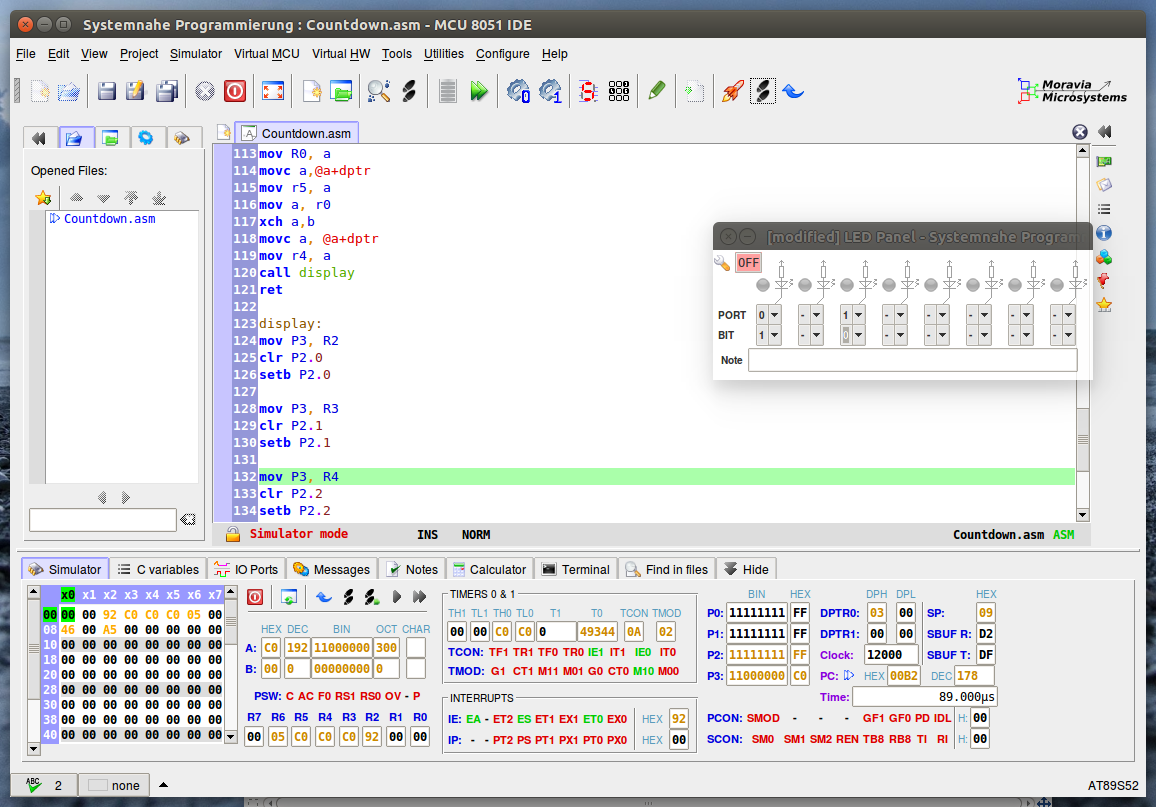
\includegraphics{images/ide.png}
\caption{MCU 8051 IDE}
\end{figure}

Zentrales Element der \ac{IDE} ist der Code Editor, welcher mit üblichen aber auch zusätzlichen
Features aufwartet. Er bietet Funktionen wie Syntax Highlighting, Vervollständigung der Befehle
während des Tippens, Überprüfung der Code Syntax und der Rechtschreibung in Kommentaren. Neben der
Anzeige von Zeilennummern, Lesezeichen und Haltemarken ist es möglich den Code als XHTML oder LaTeX
Dokument zu exportieren.

\begin{figure}[htbp]
\centering
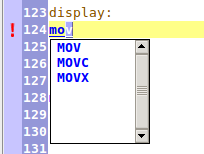
\includegraphics{images/editor.png}
\caption{MCU 8051 IDE Editor}
\end{figure}

Im unteren Bereich der \ac{IDE} ist der Simulator untergebracht. Er virtualisiert einen gewählten
Microcontroller und gibt dem Benutzer die Möglichkeit genau zu erkennen, wie sich die Kompenenten
verhalten, nachdem z.B. der Wert des Registers verändert wird. So wird es möglich bestimmte Fehler
im Programm zu finden, was mit reeler Hardware nahezu unmöglich wäre. Der Benutzer hat darüber
hinaus die Möglichkeit jegliche Speicher zu editieren und das Verhalten direkt zu beobachten. Ein
Abbild des laufenden Programms kann außerdem in einer Datei gespeichert werden und zu einem späteren
Zeitpunkt fortgesetzt werden.

Die \ac{IDE} kann zudem die geöffneten Source Code Dateien samt Konfigurationsparameter in einer
\ac{XML} Datei speichern. Der integrierte wissenschaftliche Rechner bietet unter anderem die
Umrechnung von Zahlen zwischen Hexadezimal, Dezimal, Oktal und Binär Zahlensystemen. Rohdaten können
direkt im integrierten Hexadezimal Editor bearbeitet werden. Assemblercode kann mit dem Disassembler
wieder zurück in Source Code verwandelt werden.

Neben dem Simulator stehen auch eine Zahl an Hardware Visualisierungen zur Verfügung. Mit Hilfe
dieser können \ac{LED}s, Displays oder auch Temperatursensoren an den Simulator angschlossen
werden.\footnote{(o.V.) (o.J.) MCU 8051 IDE, http://www.moravia-microsystems.com/mcu-8051-ide,
  Einsichtnahme: 28.01.2015.}

\begin{figure}[htbp]
\centering
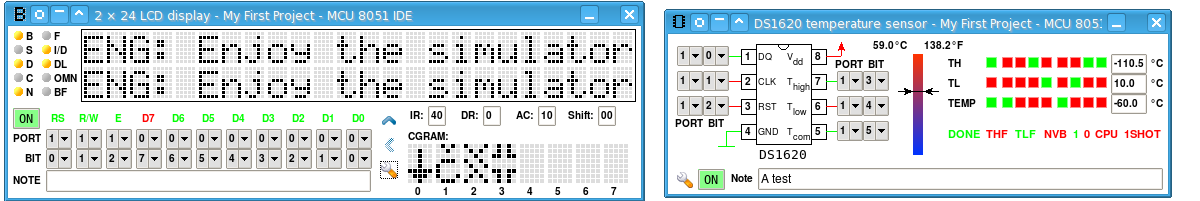
\includegraphics{images/display-temp.png}
\caption{MCU 8051 IDE Hardware Visualisierung}
\end{figure}
%!TEX root = ../systemnahe-programmierung.tex

\chapter{Projektidee}\label{projektidee}

\begin{figure}[htbp]
\centering
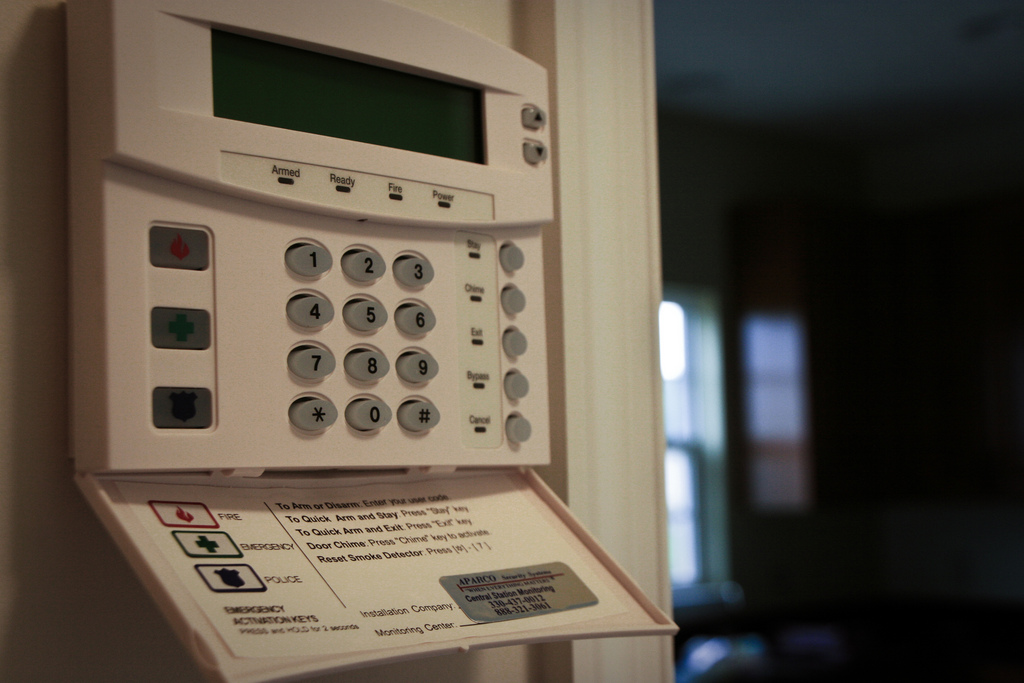
\includegraphics{images/keypad.jpg}
\caption[Nummerfeld einer Alarmsicherung]{Nummerfeld einer Alarmsicherung\footnotemark{}}
\end{figure}
\footnotetext{Quelle: https://www.flickr.com/photos/themillers91705/4916981638}

Bei einer Alarmsicherung meldet man sich normalerweise über ein Nummerfeld an, um den Alarmmodus an-
und auzuschalten. In diesem Projekt wollen wir eine einfaches Nummernfeld simulieren: Wenn man eine
vordefinierte 4-stellige Ziffernfolge eingiebt, kann man den Modus der Alarmsicherung ändern
(aus-/eingeschaltet).
%!TEX root = ../systemnahe-programmierung.tex

\chapter{Implementierung}\label{implementierung}

\begin{figure}[htbp]
\centering
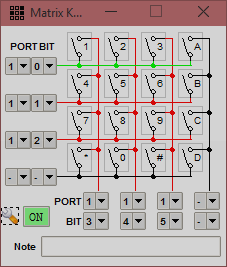
\includegraphics{images/keypad-screenshot}
\caption{Konfiguration des Nummernfeldes}
\end{figure}

Für die Simulation des Nummernfeldes wird das \emph{Matrix Keypad} der \emph{MCU 8051 IDE}
verwendet. Als Erstes muss die Pin-Belegung konfiguriert werden. Im Bild kann man sehen, dass das
Nummerfeld auf Port 1 erreichbar ist. Diese Einstellung kann auch in die IDE import werden (siehe
Anhang).

\begin{lstlisting}
keypad      equ P1              ;Matrix keypad
col1        equ keypad.3        ;Column 1
col2        equ keypad.4        ;Column 2
col3        equ keypad.5        ;Column 3

value       equ 30H             ;Value of pressed button
pressed     bit 00H             ;Was the button just pressed?
secure_mode bit 01h             ;Is the user logiged in?
\end{lstlisting}

Zusätzlich zu den Bits für das Nummernfeld werden auch noch drei Variablen definiert:

\begin{itemize}
\item
  \mintinline{text}{value}: Wert der gedrückten Taste
\item
  \mintinline{text}{pressed}: Ob schon eine Taste gedrückt wurde (wird zurückgesetzt, wenn auf ein neuen
  Tastendruck gewartet wird)
\item
  \mintinline{text}{secure_mode}: In welchem Zustand die Alarmsicherung ist (0 für ausgeschaltet, 1 für
  eingeschaltet)
\end{itemize}

\begin{lstlisting}
get_button:
    clr pressed

    ;Check first row
    mov value,#1                ;Start value is first number on row
    mov keypad, #11111110B      ;Mark first row
    acall check_col1            ;Check all columns 

    ;If button was pressed in row, jump out of function
    jb pressed, found_button    
 
    mov value,#4
    mov keypad, #11111101B
    acall check_col1
 
    jb pressed, found_button
 
    mov value,#7
    mov keypad, #11111011B
    acall check_col1
 
    jb pressed, found_button

    jmp get_button
\end{lstlisting}

Die Zeilen des Nummernfeldes werden nacheinander überprüft. Dabei wird zuerst \mintinline{text}{value} auf
den Wert der ersten Taste aus der Reihe gesetzt. Danach werden alle Reihen außer die ausgewählte auf
\mintinline{text}{1} gesetzt und zur Funktion \mintinline{text}{check_col1} gesprungen, die die Spaltenüberprüfung
für die ausgewählte Reihe startet. Nach jeder Reihe wird überprüft, ob schon eine Taste gedrückt
wird. Ist dies der Fall, dann wird aus der Funktion gesprungen. Wenn alle Reihen überprüft worden
sind und kein Tastendruck erkannt wurde, dann wird die Überprüfung wieder von vorne angefangen.

\begin{lstlisting}
check_col1:
    ;If button wasn't pressed, jump to next colum
    jb col1, check_col2

    ;If button was pressed, wait for end of button press
    jnb col1,$

    ;Set bit that key was pressed
    setb pressed
    ret
\end{lstlisting}

Wenn in der ersten Spalte kein Tastendruck entdeckt worden ist, wird zu \mintinline{text}{check_col2}
gesprungen, die die nächste Spalte überprüft. Sollte die Taste aber gedrückt sein, dass muss erst
auf das Ende des Tastendrucks gewartet werden. Dafür wird einfach zur gleichen Zeile der Überprüfung
gesprungen. Dach wird noch das Bit für \mintinline{text}{pressed} auf \mintinline{text}{1} gesetzt.

\begin{lstlisting}
check_col2:
    jb col2, check_col3
    jnb col2,$
    inc value           ;Increment the start value from row
    setb pressed
    ret
\end{lstlisting}

Die Überprüfung der nächsten Spalten funktioniert fast identisch. Der einzige Unterschied findet bei
einem erfolgreichem Tastendruck statt. Da der Wert der Taste verschiedene Werte hat, muss der Inhalt
von \mintinline{text}{value} noch angepasst werden. Dafür wird einfach um den Unterschied inkrementiert (in
diesem Fall 1).

\begin{lstlisting}
check_pin:
    ;Check first pin (4)
    acall get_button
    mov A, value
    cjne A, #4, check_pin

    ;Check second pin (2)
    acall get_button
    mov A, value
    cjne A, #2, check_pin

    ;Check third pin (6)
    acall get_button
    mov A, value
    cjne A, #6, check_pin

    ;Check fourth pin (8)
    acall get_button
    mov A, value
    cjne A, #8, check_pin

    ;Toggle secure mode of the system
    cpl secure_mode
\end{lstlisting}

Die Hauptfunktion ist \mintinline{text}{check_pin}. Sie ruft viermal die \mintinline{text}{get_button}-Funktion
auf und überprüft, ob der gelieferte Tastendruck dem gewünschtem gleicht. Sollte dies einmal nicht
der Fall sein, dann wird die Suche von vorne angefangen. Aber wurde die Ziffernfolge erfolgreich
eingegeben, dann wird der Alarm-Modus gewechselt. Die Zifferfolge lässt sich sehr leicht ändern,
unter anderem auch in der Länge.


% Anhang
\clearpage
\pagenumbering{Roman}

% Abbildungsverzeichnis
\cleardoublepage
\listoffigures

%Tabellenverzeichnis
\cleardoublepage
\listoftables

% Quellcodeverzeichnis
% \cleardoublepage
% \lstlistoflistings

% Literaturverzeichnis
\cleardoublepage
\printbibliography

% Abkürzungsverzeichnis
\cleardoublepage
%!TEX root = ../praxisbericht-docker.tex

\chapter*{Abkürzungsverzeichnis}
\phantomsection \label{listofacs}
\addcontentsline{toc}{chapter}{Abkürzungsverzeichnis}

%nur verwendete Akronyme werden letztlich im Dokument angezeigt
\begin{acronym}[YTMMM]
\setlength{\itemsep}{-\parsep}

\acro{AGPL}{Affero GNU General Public License}
\acro{API}{Application Programming Interface}
\acro{WYSIWYG}{What You See Is What You Get}
\acro{HTML}{Hypertext Meta Language}
\end{acronym}


% Glossar
\printglossary[style=altlist,title=Glossar]

\end{document}